
As mentioned in the previous section, a compiler is a complex piece of software. Collecting statistical numbers—for example, the number of basic blocks processed by a specific optimization—is one of the easiest and most efficient ways to get a quick portrait on the runtime behaviors of a compiler.

There are several ways to collect statistics in LLVM. In this section, we are going to learn three of the most common and useful options for doing this, and these methods are outlined here:

\begin{itemize}
\item Using the Statistic class
\item Using an optimization remark
\item Adding time measurements
\end{itemize}

The first option is a general utility that collects statistics via simple counters; the second option is specifically designed to profile compiler optimizations; and the last option is use for collecting timing information in the compiler.

Let's start with the first one.

\subsubsubsection{11.3.1\hspace{0.2cm}Using the Statistic class}

In this section, we are going to demonstrate new features by amending them to the SimpleMulOpt LLVM Pass from the previous section. First, let's assume that we don't only want to print out the operand Value from multiplication instructions but that we also want to count how many multiplication instructions have been processed by our Pass. First, let's try to implement this feature using the LLVM\_DEBUG infrastructure we just learned about, as follows:

\begin{lstlisting}[style=styleCXX]
#define DEBUG_TYPE "simple-mul-opt"
PreservedAnalyses
SimpleMulOpt::run(Function &F, FunctionAnalysisManager &FAM) {
	unsigned NumMul = 0;
	for (auto &I : instructions(F)) {
		if (auto *BinOp = dyn_cast<BinaryOperator>(&I) &&
		BinOp->getOpcode() == Instruction::Mul) {
			++NumMul;
			…
		}
	}
	LLVM_DEBUG(dbgs() << "Number of multiplication: " << NumMul);
	…
}
\end{lstlisting}

This approach seems pretty straightforward. But it comes with a drawback—the statistical numbers we are interested in are mixed with other debug messages. We need to take additional actions to parse or filter the value we want because although you might argue that these problems could be tackled by using a separate DEBUG\_TYPE tag for each counter variable, when the number of counter variables increases, you might find yourself creating lots of redundant code.

One elegant solution is to use the Statistic class (and related utilities) provided by LLVM. Here is a version rewritten using this solution:

\begin{lstlisting}[style=styleCXX]
#include "llvm/ADT/Statistic.h"
#define DEBUG_TYPE "simple-mul-opt"
STATISTIC(NumMul, "Number of multiplications processed");
PreservedAnalyses
SimpleMulOpt::run(Function &F, FunctionAnalysisManager &FAM) {
	for (auto &I : instructions(F)) {
		if (auto *BinOp = dyn_cast<BinaryOperator>(&I) &&
		BinOp->getOpcode() == Instruction::Mul) {
			++NumMul;
			…
		}
	}
	…
}
\end{lstlisting}

The preceding code snippet shows the usage of Statistic, calling the STATISTIC macro function to create a Statistic type variable (with a textual description) and simply using it like a normal integer counter variable.

This solution only needs to modify a few lines in the original code, plus it collects all counter values and prints them in a table view at the end of the optimization. For example, if you run the SimpleMulOpt Pass using the -stats flag with opt, you will get the following output:

\begin{tcblisting}{commandshell={}}
$ opt -stats –load-pass-plugin=… …
===-------------------------------===
      … Statistics Collected …
===-------------------------------===
87 simple-mul-opt - Number of multiplications processed
$
\end{tcblisting}

87 is the number of multiplication instructions processed in SimpleMulOpt. Of course, you are free to add as many Statistic counters as you want in order to collect different statistics. If you run more than one Pass in the pipeline, all of the statistical numbers will be presented in the same table. For instance, if we add another Statistic counter into SimpleMulOpt to collect a number of none-power-of-two constant operands from the multiplication instructions and run the Pass with Scalar Replacement of Aggregates (SROA), we can get an output similar to the one shown next:

\begin{tcblisting}{commandshell={}}
$ opt -stats –load-pass-plugin=… --passes="sroa,simple-multopt" …
===-------------------------------===
       … Statistics Collected …
===-------------------------------===
94 simple-mul-opt - Number of multiplications processed
87 simple-mul-opt - Number of none-power-of-two constant
operands
100 sroa - Number of alloca partition uses rewritten
34 sroa - Number of instructions deleted
… 
$
\end{tcblisting}

The second column in the preceding code snippet is the name of the origin Pass, which is designated by the DEBUG\_TYPE value defined prior to any calls to STATISTIC.

Alternatively, you can output the result in JavaScript Object Notation (JSON) format by adding the -stats-json flag to opt. For example, look at the following code snippet:

\begin{tcblisting}{commandshell={}}
$ opt -stats -stats-json –load-pass-plugin=… …
{
	"simple-mul-opt.NumMul": 87
}
$
\end{tcblisting}

In this JSON format, instead of printing statistic values with a textual description, the field name of a statistic entry has this format: "<Pass name>.<Statistic variable name>" (the Pass name here is also the value of DEBUG\_TYPE). Furthermore, you can print statistic results (either in default or JSON format) into a file using the -infooutput-file=<file name> command-line option. The following code snippet shows an example of this:

\begin{tcblisting}{commandshell={}}
$ opt -stats -stats-json -info-output-file=my_stats.json …
$ cat my_stats.json
{
	"simple-mul-opt.NumMul": 87
} 
$
\end{tcblisting}

You have now learned how to collect simple statistic values using the Statistic class. In the next section, we are going to learn a statistic collecting method that is unique to compiler optimization.

\subsubsubsection{11.3.2\hspace{0.2cm}Using an optimization remark}

A typical compiler optimization usually consists of two stages: searching for the desired patterns from the input code, followed by modifying the code. Take our SimpleMulOpt Pass as an example: the first stage is to look for multiplication instructions (BinaryOperator with the Instruction::Mul operation code (opcode)) with power-of-two constant operands. For the second stage, we create new left-shifting instructions via IRBuilder::CreateShl(…) and replace all old usages of multiplication instructions with these.

There are many cases, however, where the optimization algorithm simply "bails out" during the first stage due to infeasible input code. For example, in SimpleMulOpt, we are looking for a multiplication instruction, but if the incoming instruction is not BinaryOperator, the Pass will not proceed to the second stage (and continue on to the next instruction). Sometimes, we want to know the reason behind this bailout, which can help us to improve the optimization algorithm or diagnose incorrect/suboptimal compiler optimization. LLVM provides a nice utility called an optimization remarks to collect and report this kind of bailout (or any kind of information) occurring in optimization Passes.

For example, let's assume we have the following input code:

\begin{lstlisting}[style=styleCXX]
int foo(int *a, int N) {
	int x = a[5];
	for (int i = 0; i < N; i += 3) {
		a[i] += 2;
		x = a[5];
	}
	return x;
}
\end{lstlisting}

Theoretically, we can use loop-invariant code motion (LICM) to optimize this code into an equivalent code base such as this one:

\begin{lstlisting}[style=styleCXX]
int foo(int *a, int N) {
	for (int i = 0; i < N; i += 3) {
		a[i] += 2;
	}
	return a[5];
}
\end{lstlisting}

We can do this as the fifth array element, a[5], never changed its value inside the loop. However, if we run LLVM's LICM Pass over the original code, it fails to perform the expected optimization.

To diagnose this problem, we can invoke the opt command with an additional option: -\,-pass-remarks-output=<filename>. The filename will be a YAML Ain't Markup Language (YAML) file in which optimization remarks print out the possible reasons why LICM failed to optimize. Here is an example of this:

\begin{tcblisting}{commandshell={}}
$ opt -licm input.ll –pass-remarks-output=licm_remarks.yaml …
$ cat licm_remarks.yaml
…
--- !Missed
Pass:            licm
Name:            LoadWithLoopInvariantAddressInvalidated
Function:        foo
Args:
  - String:      failed to move load with loop-invariant
address because the loop may invalidate its value
...
$
\end{tcblisting}

The cat command in the preceding output shows one of the optimization remark entries in licm\_remarks.yaml. This entry tells us that there was a missed optimization that happened in the LICM Pass when it was processing the foo function. It also tells us the reason: LICM was not sure if a particular memory address was invalidated by the loop. Though this message doesn't provide fine-grained details, we can still infer that the problematic memory address concerning LICM was probably a[5]. LICM was not sure if the a[i] += 2 statement modified the content of a[5].

With this knowledge, compiler developers can get hands-on in improving LICM—for example, teaching LICM to recognize induction variables (that is, the i variable in this loop) with a step value greater than 1 (in this case, it was 3, since i += 3).

To generate optimization remarks such as the one shown in the preceding output, compiler developers need to integrate a specific utility API into their optimization Pass. To show you how to do that in your own Pass, we are going to reuse our SimpleMulOpt Pass as the sample. Here is part of the code that performs the first stage—searching for multiplications with power-of-two constant operands—in SimpleMulOpt:

\begin{lstlisting}[style=styleCXX]
…
for (auto &I : instructions(F)) {
	if (auto *BinOp = dyn_cast<BinaryOperator>(&I))
	if (BinOp->getOpcode() == Instruction::Mul) {
		auto *LHS = BinOp->getOperand(0),
		     *RHS = BinOp->getOperand(1);
		// Has no constant operand
		if (!isa<Constant>(RHS)) continue;
		const APInt &Const = cast<ConstantInt>(RHS)->getValue();
		// Constant operand is not power of two
		if (!Const.isPowerOf2()) continue;
		…
	}
}
\end{lstlisting}

The preceding code checks if the operand is constant before making sure it's  also a powerof-two operand. If either of these checks fails, the algorithm will bail out by continuing on to the next instruction in the function.

We intentionally inserted a small flaw into this code to make it less powerful, and we are going to show you how to find that problem by using an optimization remark. Here are the steps to do this:

\begin{enumerate}
\item First, we need to have an OptimizationRemarkEmitter instance, which can help you to emit remark messages. This can be obtained from its parent analyzer, OptimizationRemarkEmitterAnalysis. Here is how we include it at the beginning of the SimpleMulOpt::run method:

\begin{lstlisting}[style=styleCXX]
#include "llvm/Analysis/OptimizationRemarkEmitter.h"
PreservedAnalyses
SimpleMulOpt::run(Function &F, FunctionAnalysisManager
&FAM) {
	OptimizationRemarkEmitter &ORE
	  = FAM.getResult<OptimizationRemarkEmitterAnalysis>(F);
	…
}
\end{lstlisting}

\item Then, we are going to use this OptimizationRemarkEmitter instance to emit an optimization remark if the multiplication instruction lacks a constant operand, as follows:

\begin{lstlisting}[style=styleCXX]
#include "llvm/IR/DiagnosticInfo.h"
…
if (auto *BinOp = dyn_cast<BinaryOperator>(&I))
if (BinOp->getOpcode() == Instruction::Mul) {
	auto *LHS = BinOp->getOperand(0),
	*RHS = BinOp->getOperand(1);
	// Has no constant operand
	if (!isa<ConstantInt>(RHS)) {
		std::string InstStr;
		raw_string_ostream SS(InstStr);
		I.print(SS);
		ORE.emit([&]() {
			return OptimizationRemarkMissed(DEBUG_TYPE,
				"NoConstOperand", &F)
				<< "Instruction" <<
				<< ore::NV("Inst", SS.str())
				<< " does not have any constant operand";
			});
			continue;
		}
	}
…
\end{lstlisting}

There are several things to be noticed here, as follows:

\begin{itemize}
\item The OptimizationRemarkEmitter::emit method takes a lambda function as the argument. This lambda function will be invoked to emit an optimization remark object if the optimization remark feature is turned on (via the –passremarks-output command-line option we've seen previously, for example).

\item The OptimizationRemarkMissed class (note that it is not declared in
OptimizationRemarkEmitter.h but in the DiagnosticInfo.h header file) represents the remark of a missed optimization opportunity. In this case, the missed opportunity is the fact that instruction I does not have any constant operand. The constructor of OptimizationRemarkMissed takes three arguments: the name of the Pass, the name of the missed optimization opportunity, and the enclosing IR unit (in this case, we use the enclosing Function). In addition to constructing a OptimizationRemarkMissed object, we also concatenate several objects via the stream operator (<<) at the tail. These objects will eventually be put under the Args section of each optimization remark entry in the YAML file we saw previously.

In addition to using OptimizationRemarkMissed to notify you of missed optimization opportunities, you can also use other classes derived from DiagnosticInfoOptimizationBase to present different kinds of information—for example, use OptimizationRemark to find out which optimization has been successfully applied, and use OptimizationRemarkAnalysis to keep a log of analysis data/facts.

\item Among objects concatenated by the stream operator, ore::NV(…) seems to be a special case. Recall that in the optimization remark YAML file, each line under the Args section was a key-value pair (for example, String: failed to move load with…., where String was the key). The ore::NV object allows you to customize the key-value pair. In this case, we are using Inst as the key and SS.str() as the value. This feature provides more flexibility to parse the optimization remark YAML file—for instance, if you want to write a little tool to visualize the optimization remarks, custom Args keys can give you an easier time (during the parsing stage) by distinguishing critical data from other strings.

\end{itemize}

\item Now that you have inserted the code to emit the optimization remark, it's time to test it. This time, we are going to use the following IR function as the input code:

\begin{lstlisting}[style=styleCXX]
define i32 @bar(i32 %0) {
	%2 = mul nsw i32 %0, 3
	%3 = mul nsw i32 8, %3
	ret %3
}
\end{lstlisting}

You can rebuild the SimpleMulOpt Pass and run it using a command such as this:

\begin{tcblisting}{commandshell={}}
$ opt –load-pass-plugin=… –passes="simple-mul-opt" \
–pass-remarks-output=remark.yaml -disable-output
input.ll
$ cat remark.yaml
--- !Missed
Pass:        simple-mul-opt
Name:        NoConstOperand
Function:    bar
Args:
  - String:  'Instruction'
  - Inst:    ' %3 = mul nsw i32 8, %3'
  - String:  ' does not contain any constant
operand'
...
$
\end{tcblisting}

From this optimization remark entry, we can glean that SimpleMulOpt bailed out because it couldn't find a constant operand on one of the (multiplication) instructions. The Args section shows a detailed reason for this.

With this information, we realize that SimpleMulOpt is unable to optimize a multiplication whose first operand (LHS operand) is a power-of-two constant, albeit a proper optimization opportunity. Thus, we can now fix the implementation of SimpleMulOpt to check if either of the operands is constant, as follows:

\begin{lstlisting}[style=styleCXX]
…
if (BinOp->getOpcode() == Instruction::Mul) {
	auto *LHS = BinOp->getOperand(0),
	*RHS = BinOp->getOperand(1);
	// Has no constant operand
	if (!isa<ConstantInt>(RHS) && !isa<ConstantInt>(LHS)) {
		ORE.emit([&]() {
			return …
		});
		continue;
	}
	…
} …
\end{lstlisting}

You have now learned how to emit optimization remarks in an LLVM Pass and how to use the generated report to discover potential optimization opportunities.

\end{enumerate}

So far, we have only studied the generated optimization remark YAML file. Though it has provided valuable diagnostic information, it would be great if we could have more fine-grained and intuitive location information to know where exactly these remarks happened. Luckily, Clang and LLVM have provided a way to achieve that.

With the help of Clang, we can actually generate optimization remarks with source location (that is, line and column numbers in the original source file) attached. Furthermore, LLVM provides you with a small utility that can associate an optimization remark with its corresponding source location and visualize the result on a web page. Here's how to do this:

\begin{enumerate}
\item Let's reuse the following code as the input:

\begin{lstlisting}[style=styleCXX]
int foo(int *a, int N) {
	for (int i = 0; i < N; i += 3) {
		a[i] += 2;
	}
	return a[5];
}
\end{lstlisting}

First, let's generate optimization remarks using this clang command:

\begin{tcblisting}{commandshell={}}
$ clang -O3 -foptimization-record-file=licm.remark.yaml \
        -S opt_remark_licm.c
\end{tcblisting}

Though we're using a different name, -foptimization-record-file is the command-line option used to generate an optimization remark file with the given filename.

\item After licm.remark.yaml is generated, let's use a utility called opt-viewer.py to visualize the remarks. The opt-viewer.py script is not installed in the typical location by default—instead of putting it in <install path>/bin (for example /usr/bin), it is installed in <install path>/share/opt-viewer (/usr/share/opt-viewer). We are going to invoke this script with the following command-line options:

\begin{tcblisting}{commandshell={}}
$ opt-viewer.py --source-dir=$PWD \
--target-dir=licm_remark licm.remark.yaml
\end{tcblisting}

(Note that opt-viewer.py depends on several Python packages such as pyyaml and pygments. Please install them before you use opt-viewer.py.)

\item There will be a HTML file—index.html—generated inside the licm\_remark folder. Before you open the web page, please copy the original source code—opt\_remark\_licm.c—into that folder as well. After that, you will be able to see a web page like this:

\hspace*{\fill} \\ %插入空行
\begin{center}
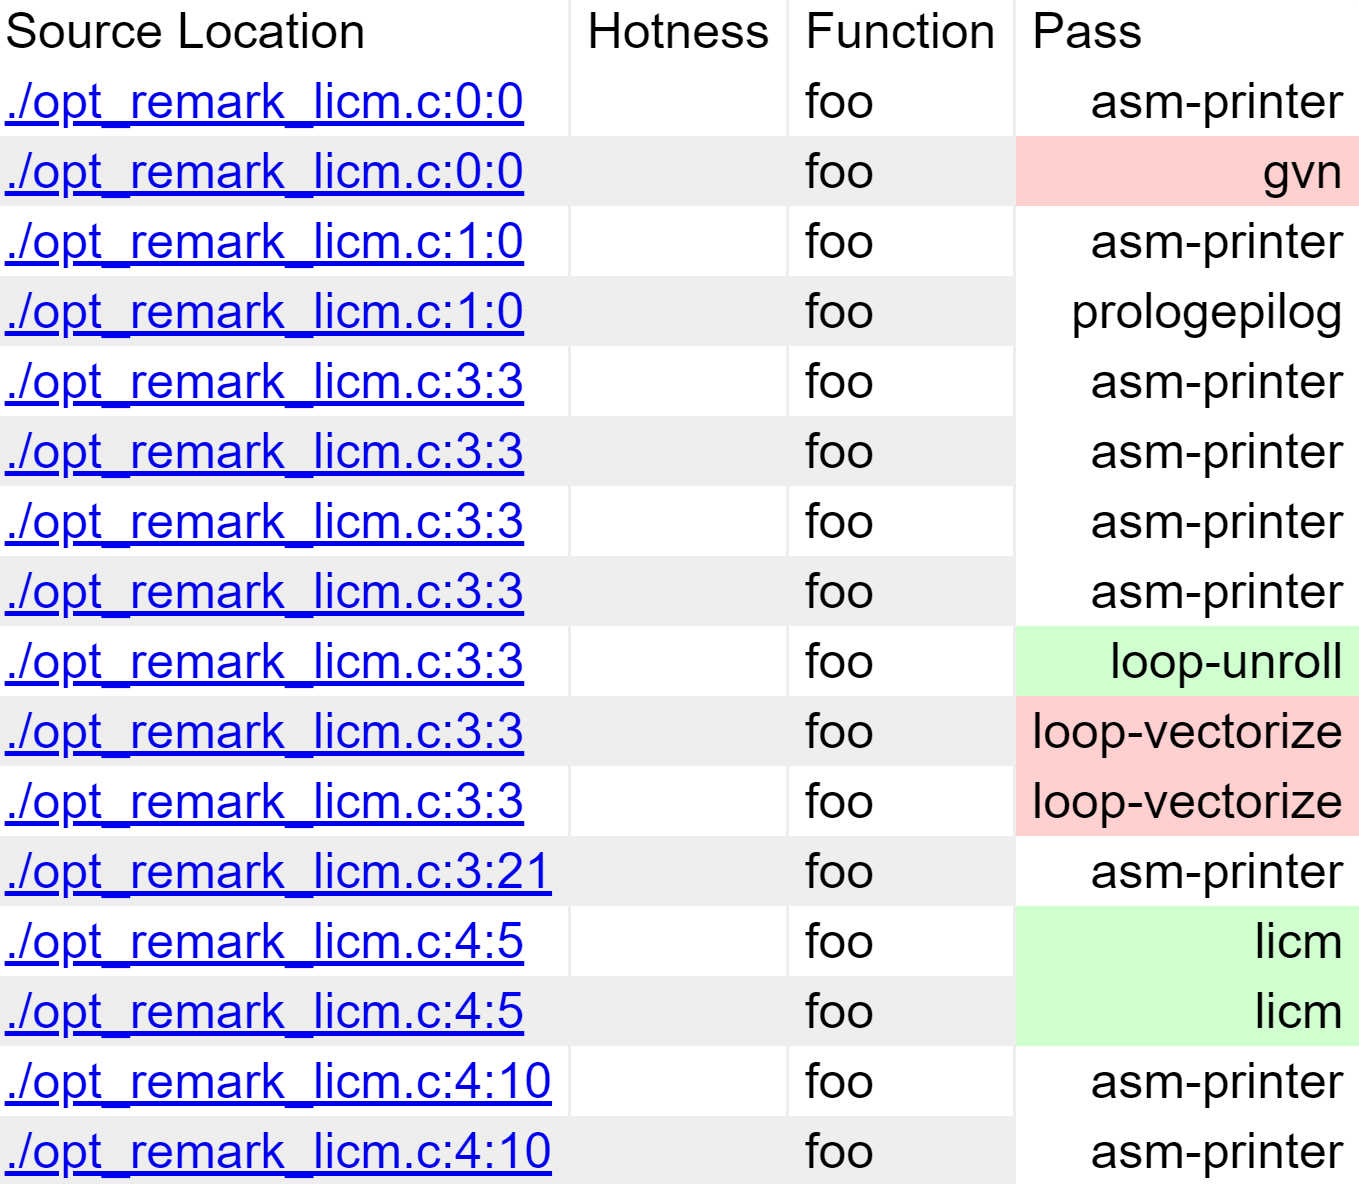
\includegraphics[width=0.9\textwidth]{content/3/chapter11/images/1.png}\\
Figure 11.1 – Web page of optimization remarks combined with the source file
\end{center}

We are particularly interested in two of these columns: Source Location and Pass. The latter column shows the name of the Pass and the type of the optimization remark—Missed, Passed, or Analyzed rendered in red, green, and white, respectively—attached on a given line shown at the Source Location column.

If we click on a link in the Source Location column, this will navigate you to a page that looks like this:

\hspace*{\fill} \\ %插入空行
\begin{center}
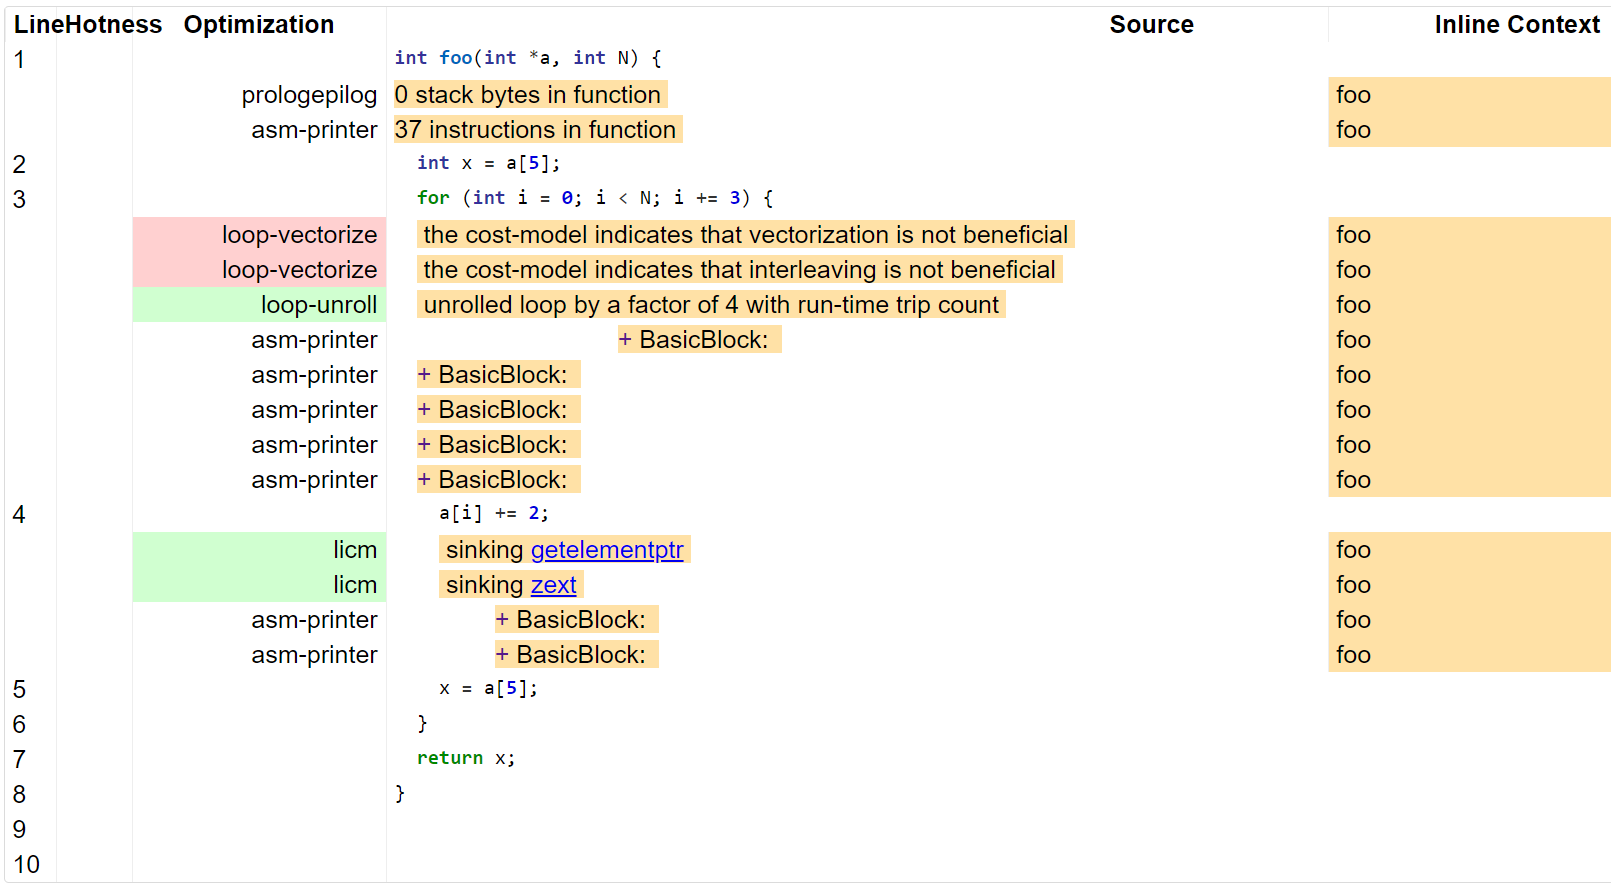
\includegraphics[width=0.9\textwidth]{content/3/chapter11/images/2.png}\\
Figure 11.2 – Details of an optimization remark
\end{center}

This page gives you a nice view of optimization remark details, interleaved with the originating source code line. For example, on line 3, loop-vectorize Pass said it couldn't vectorize this loop because its cost model didn't think it was beneficial to do so.

\end{enumerate}

You have now learned how to use optimization remarks to gain insights into the optimization Pass, which is especially useful when you're debugging a missing optimization opportunity or fixing a mis-compilation bug.

In the next section, we are going to learn some useful skills to profile the execution time of LLVM.





















